%
% latex-sample.tex
%
% This LaTeX source file provides a template for a typical research paper.
%

%
% Use the standard article template.
%
\documentclass{article}

% The geometry package allows for easy page formatting.
\usepackage{geometry}
\geometry{letterpaper}

% Load up special logo commands.
\usepackage{doc}

% Package for formatting URLs.
\usepackage{url}

% Packages and definitions for graphics files.
\usepackage{graphicx}
\usepackage{epstopdf}
\DeclareGraphicsRule{.tif}{png}{.png}{`convert #1 `dirname #1`/`basename #1 .tif`.png}

%
% Set the title, author, and date.
%
\title{Usability of Modern Display Technologies}
\author{Rachel Rivera}
\date{October 16, 2014}

%
% The document proper.
%
\begin{document}

% Add the title section.
\maketitle

% Add an abstract.
\abstract{
This study aims to examine how interaction design concepts specifically map to the usability of modern display technology.
//TODO: write a better abstract
}

% Add various lists on new pages.
\pagebreak
\tableofcontents


% Start the paper on a new page.
\pagebreak

%
% Body text.
%
\section{Introduction}
\label{introduction}

You will almost certainly start with an introductory description of the topic that you investigated in your assignment.  Discuss any goals, motivation, or examples of the subject; the key is to provide the reader with any information that is necessary to understand why your topic was worth investigating.  This descriptive section should also allow the reader to understand the subsequent detail sections on the subject.

\section{Background, Preliminary, and Related Work}

Perhaps the most important functionality to learn for the paper is \LaTeX\ bibliography support.  Citations and references are handled automatically by \LaTeX\ through its companion program, \BibTeX.  All you have to do is provide a bibliography file that provides the reference information and internal keys (very much like variable names) that you use in your document.\footnote{And always remember to run \LaTeX\ \emph{at least twice} after running \BibTeX.}

\BibTeX\ supports virtually all kinds of references, including books \cite{dui,sgg,iokit,palmos}, parts of books \cite{userModeLinux}, articles \cite{nielsen:dui-review,heer-shneiderman,stackableThreads,xpkernel}, and conference proceedings \cite{ux-3d,iring,contextFileSearch,osHaskell,hibernator}, to name a few.  If not already included in your \LaTeX\ distribution, download and install the \texttt{url} package to support formatting of URLs; you can usually mention these in the \emph{note} or \emph{howpublished} fields of your \BibTeX\ file.

Like Section~\ref{introduction}, a background, preliminary, and related work section is also almost certainly needed for your paper.  In this section, describe any history, work, or projects that serve as direct contributors to the subject of your research paper.  Look at other papers in the literature to see how they organized, presented, and discussed prior work.

The Shneiderman/Plaisant text \cite{dui} provide some pointers to seminal or key works; because they made it into the textbook they aren't necessarily ``bleeding edge,'' but they likely provide the foundation for your chosen subject matter.

\section{Main Content Sections}

The outline after the introductory and background, preliminary, and related work sections is more dependent on the specific subject of your research.  Remember to cite references where appropriate, organize the material so that it flows well and is clear to the reader.

\subsection{Multiple Outline Levels}

\LaTeX\ has support for up to three outline levels (\verb!\section!, \verb!\subsection!, and \verb!\subsubsection!).  It also recognizes \verb!\paragraph! and \verb!\subparagraph! directives, though those don't show up in the table of contents.  All of these directives expect a title.

Note also the use of the \verb!\verb! directive for inserting code-like labels or symbols.  It was particularly needed here so that we can include the backslash character in the text.

\subsection{Tables and Figures}

\LaTeX\ has full support for tables and figures.  Table~\ref{table-sample} shows a sample table and Figure~\ref{figure-sample} shows a sample figure.  Note the built-in support for captions and the automated numbering functionality.  Lists of tables and figures can also be automatically generated, as seen at the beginning of this document.

\begin{table}
\centering
\begin{tabular}{|c|c|c|}\hline
Column 1 & Column 2 & Column 3 \\\hline\hline
a & b & c \\
d & e & f \\
g & h & i \\\hline
\end{tabular}

\caption{A sample table}
\label{table-sample}
\end{table}

\begin{figure}
\centering
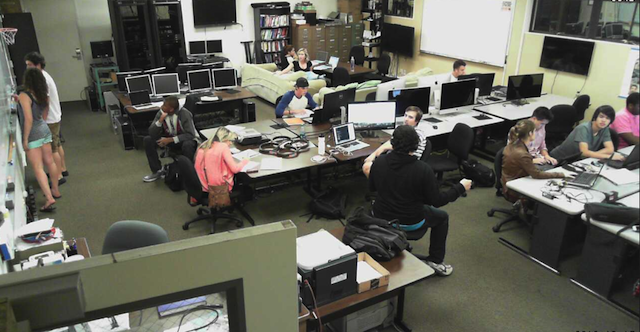
\includegraphics[width=2in]{space.jpg} 

\caption{A sample figure}
\label{figure-sample}
\end{figure}

One very important thing to remember about how \LaTeX\ handles tables and figures by default: you don't have to worry about where they go exactly.  The general rule is that you insert them in the source after your first reference to them, and \LaTeX\ determines their final position.  It also makes decisions on how much page space to devote to them.  This all follows \LaTeX's overall theme of focusing on the content of your paper, and not its format.

Just so you can see a second table, Table~\ref{table-sample2} is provided.

\begin{table}
\centering
\begin{tabular}{|c|c|c|}\hline
Column 1 & Column 2 & Column 3 \\\hline\hline
a & b & c \\
d & e & f \\
g & h & i \\\hline
\end{tabular}

\caption{Another sample table}
\label{table-sample2}
\end{table}

\section{Another Section}

We're adding another section just so you can see how that looks.  Plus there are a few more \LaTeX\ features to illustrate.

\subsection{Bulleted and Numbered Lists}

\LaTeX\ is very good at providing clean lists.  Examples are shown below.

\begin{itemize}
\item Bulleted items come out properly indented and spaced, every time.

\begin{itemize}
\item Sub-bullets are a virtual no-brainer: just nest another \verb!itemize! block.
\item Note how the bullet character automatically changes too.
\end{itemize}

\item Just keep on adding \verb!\item!s\ldots

\item \ldots until you're done.
\end{itemize}

Numbered lists are almost identical, except that you specify \verb!enumerate! instead of \verb!itemize!.  List items are specified in exactly the same way (thus making it easy to change list types).

\begin{enumerate}
\item A list item
\item Another list item
\item A list item with multiple nested lists

\begin{itemize}
\item Nested lists can be of mixed types.
\item That's a lot of power and flexibility for the price of learning a handful of directives.

\begin{enumerate}
\item Like nested bullet lists, nested numbered lists also ``intelligently'' change their numbering schemes.
\item Meanwhile, all \emph{you} have to write is \verb!\item!.  \LaTeX\ does the rest.
\end{enumerate}
\end{itemize}

\item Back to your regularly scheduled list item

\end{enumerate}

\subsection{Subsection with Another Figure}

We may as well include a second figure also, shown in Figure~\ref{figure-sample2}.  The same image file is used, but note how it can be resized.  Again, observe how the positions of the tables and figures do not necessarily match their positions in the source file, reiterating the aforementioned \LaTeX\ functionality for deciding where these items go in the final document.  You provide an approximate location, and \LaTeX\ does the rest.

\begin{figure}
\centering
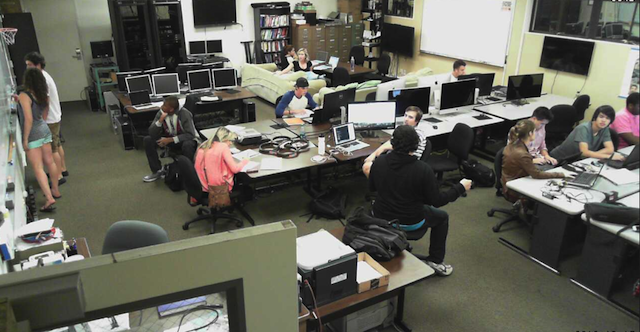
\includegraphics[width=1in]{space.jpg} 

\caption{Another sample figure}
\label{figure-sample2}
\end{figure}

\section{Conclusion}

Wrap up your paper with an ``executive summary'' of the paper itself, reiterating its subject and its major points.  If you want examples, just look at the conclusions from the literature.

% Generate the bibliography.
\bibliography{latex-sample}
\bibliographystyle{unsrt}

\end{document}
